\documentclass[a4paper,14pt,href]{article}

% Используем нестандартный размер шрифта
\usepackage{extsizes}

% Делаем отступ для первого параграфа
\usepackage{indentfirst}

% Для поддержки поиска по pdf документу
\usepackage{cmap}

% Поддержка кириллицы
\usepackage[T2A]{fontenc}
\usepackage[utf8]{inputenc}
\usepackage[english,russian]{babel}

% Поддержка списков
\usepackage{enumerate}

% Заменяем библиографию с квадратных скобок на точку
\makeatletter
\renewcommand{\@biblabel}[1]{#1.}
\makeatother

% Графический пакет
\usepackage{graphicx}
\usepackage{epstopdf}
\usepackage{tikz}

% Математические шрифты AMS
\usepackage{amstext, amssymb, amsmath}

% В заголовках появляется точка, но при ссылке на них ее нет
\usepackage{misccorr}

% Поддержка гиперссылок
\usepackage{url}

% Задаем полуторный межстрочный интервал
\linespread{1.3}

% Задаем глубину оглавления
\setcounter{tocdepth}{2}

% Путь к изображениям, по умолчанию
\graphicspath{{images/}}

% Задаем отступ абзаца
\setlength{\parindent}{1.25cm}

\renewcommand{\labelenumi}{\arabic{enumi}.}% Меняем везде перечисления на цифра.цифра

% Меняем поля страницы
\usepackage{geometry}
\geometry{left=2.5cm}   % левое поле
\geometry{right=2.5cm}  % правое поле
\geometry{top=2.5cm}    % верхнее поле
\geometry{bottom=2.5cm} % нижнее поле

\begin{document}

\thispagestyle{empty}
\begin{center}
Федеральное государственное автономное образовательное учреждение \\
высшего профессионального образования \\
\textsc{<<Южный Федеральный Университет>>}\\[1.0cm]

Факультет математики, механики и компьютерных наук\\[1.0cm]

Направление подготовки 010501 --- <<Прикладная математика и информатика>>\\[3cm]

\textsc{Тестирование черного ящика на предмет анализа граничных значений}\\[3cm]

\begin{flushright}
   	Выпускная квалификационная работа \\
   	на степень бакалавра \\
   	студента \\
   	Алексея Алексеевича Тактарова \\[1.0cm]

   	Научный руководитель: \\
	доцент, к.т.н. \\
	Роман Ахмедович Хади
\end{flushright}

\vfill

	Ростов-на-Дону\\
	2012
\end{center}

\newpage
\tableofcontents

\newpage
\section*{Введение}
\addcontentsline{toc}{section}{Введение}

  Способность ошибаться, к сожалению, является неотьемлемой частью человеческой природы. Следовательно, любое изделие или продукт, произведенный человеком, может содержать ошибки, т.е. не соответствовать тем требованиям, которые были заложены в модель до изготовления. В эпоху ручного труда качество производства полностью определялось квалификацией мастера, что объясняло длительность и трудоемкость ремесленных процессов того времени. Развитие промышленности и появление конвейерного производства способствовали возникновению принципиально новых методов контроля качества, которые впоследствии легли в основу полноценной научной теории\cite{Ishikawa}.

  С появлением электронной вычислительной техники изменилась и форма продукта производства. Возникли такие отрасли, как программная инженерия, проектирование и разработка программного обеспечения, конечным результатом которых является компьютерная программа, т.е. информация.

  Нельзя, тем не менее, считать, что области, связанные с разработкой программного обеспечения, свободны от человеческих ошибок. Классическим примером, который иллюстрирует роль контроля качества в процессе проектирования компьютерных программ и систем, является неудачный запуск космического аппарата ``Маринер-1'' в 1962 году: пропущенный дефис в программе бортового компьютера стал причиной крушения аппарата, что привело к провалу всего проекта стоимостью 20 миллионов долларов\cite{Mariner}.

  В настоящее время существуют разные методы оценки качества программного обеспечения, которые могут применяться в течение всего так называемого ``жизненного цикла'' проекта. Наиболее распространенным среди разработчиков является тестирование, в основе которого лежит проверка программы на соответствие заданным требованиям посредством ряда тестов. Практика тестирования программного обеспечения получила широкое распространение благодаря своей эффективности, а в некоторых методиках разработки даже стала предшествовать написанию кода программ (Test Driven Development или TDD --- ``разработка через тестирование''\cite{ExtremeProgramming}).

  Таким образом, тестирование программного обеспечения является актуальным средством контроля качества разработки, благодаря которому возможно создание высокоэффективных отказоустойчивых программных продуктов.

\section*{Объект, предмет и цель исследования}
\addcontentsline{toc}{section}{Объект, предмет и цель исследования}
	Данная работа посвящена проблеме контроля качества программного обеспечения, в частности, проблеме проверки конечного продукта разработки на соответствие поставленным требованиям и существующим стандартам в условиях отсутствия исходных текстов.

	Предметом исследования является метод черного ящика для поиска ошибок в программном обеспечении.

	Цель работы заключается в создании программного средства, позволяющего выполнять автоматическое стресс--тестирование программ с использованием метода черного ящика.

  Были поставлены задачи, выполнение которых необходимо для достижения данной цели:
\begin{enumerate}
\item Рассмотрение современных методов контроля качества программного обеспечения.
\item Исследование существующих форм тестирования, выбор наиболее подходящей модели для практической реализации при заданных условиях.
\item Разработка программного продукта на основе выбранного метода.
\item Анализ полученных результатов.
\end{enumerate}

\section{Методы тестирования программного обеспечения}
\subsection{Верификация, валидация и тестирование}
 В основе теории, занимающейся оценкой качества программного обеспечения, лежат три понятия, которые на первый взгляд являются довольно близкими по значению: верификация, валидация и тестирование. В результаты схожести этих терминов, многие авторы интерпретируют их по-разному\cite{IntelVerification}, что является недопустимым. Дадим развернутые определения каждого из понятий.

 Верификация --- это проверка соответствия результатов отдельных этапов разработки программной системы требованиям и ограничениям. Задача верификации --- убедиться, что программное обеспечение, является функциональным, надежным, производительным, переносимым и отличается удобством сопровождения\cite{Kulyamin} \cite{ISO9126}.

 Под валидацией понимают процесс проверки того, что требования заказчика(или пользователя) системы удовлетворены. Чаще всего валидация выполняется уже после разработки и рассматривает качество программного обеспечения с точки зрения конечного потребителя.

 Наконец, тестирование является методом, при помощи которого валидация или верификация могут быть достигнуты. Однако иногда полная проверка соответствия на практике может быть невозможной, в таком случае задача тестирования --- показать, что какое-то из требований не выполняется\cite{Ahin}.

\subsection{Эффективность тестирования при оценке качества}
  Рассмотрим основные технологии контроля качества программного обеспечения:
\begin{enumerate}
\item
	\textit{Статический анализ исходного кода} используется при разработке для выявления ошибок в текстах программы на некотором языке программирования. Для этого применяются: синтаксический разбор, поиск определенных шаблонов и подозрительных мест в коде. К сожалению, данный подход является нечуствительным к ошибкам времени выполнения, кроме того он оказывается малоэффективным при работе с языками, имеющими динамическую типизацию.
\item
	\textit{Формальная верификация}	 представляет собой довольно трудозатратный метод проверки программы на соответствие некоторой математической модели. Различают дедуктивный и модельный способы верификации.

	Модельная верификация основывается на представлении программы в виде машины или автомата. Данный подход позволяет проводить не только полную, но и частичную верификацию которая может быть направлена на проверку только одного небольшого свойства, абстрагировавшись от менее важных деталей системы\cite{OpenSystems}.

	При использовании дедуктивной верификации программа воспринимается как булевская функция многих переменных $f(x_1,x_2,...,x_n)$, цель исследования при этом заключается в доказательстве, является ли данная функция выполнимой, т.е. существует ли такой набор данных $(\tilde{x_1}, \tilde{x_2}, ..., \tilde{x_n})$, что:
	$$ f(\tilde{x_1}, \tilde{x_2}, ..., \tilde{x_n}) \equiv 1 $$
Разрешением данной проблемы занимается теория SAT (Satisfiability Modulo Theories), в которой применяются так называемые \linebreak SAT--решатели, позволяющие выполнять доказательство, не прибегая к полному перебору.

 Исследованием задач подобного рода занимаются научные отделы крупных корпораций, для которых поддержание качества программного обеспечения имеет огромное значение. Примером может служить закрытая система под названием ``SAGE'', разрабатываемая Microsoft Research для внутреннего использования\cite{SAGE}.

\item
	\textit{Тестирование} является методом, при котором о качестве продукта (объекта тестирования) можно судить по результатам конечного числа тестов --- специально выбранных сценариев для проверки объекта. В отличие от статического анализа, тестирование может быть проведено на этапе выполнения программы(динамическое тестирование). Кроме того, в некоторых случая для проведения тестов необязательно знать о внутреннем устройстве программы (такой метод тестирования называется функциональным тестированием или тестированием черного ящика\cite{TestingBlackBox} \cite{TestingComputerSoftware}).
\end{enumerate}

   Таким образом, в условиях отсутствия исходных текстов тестирование является наиболее эффективным методом оценки качества программного обеспечения.
\newpage
\subsection{Модель тестирования}
\label{TestingModel}
  Центральной сущностью в тестировании является \textit{объект}, т.е. программа. Объект тестирования помещается в окружение, которое определяется конкретным тестом. При этом выдвигается некоторое предположение о том, каким будет конечное состояние объекта (после прохождения теста). Совокупность этих предположений формирует \textit{эталонную модель}. Настоящим же результатом теста может быть либо соответствие модели, либо некоторый \textit{симптом} (рисунок \ref{fig:TestingModel}).

\begin{figure}[htbp]
\begin{center}
	\includegraphics[scale=1.0]{testing_model.pdf}
    \caption{Модель тестирования}
    \label{fig:TestingModel}
\end{center}
\end{figure}

	Симптомом(или сбоем), согласно стандарту IEEE94, называют наблюдаемое аномальное поведение объекта, такое как несоответствие требованием или возникновение незапланированных явлений. Причиной симптома является \textit{сбой}, т.е. некорректное состояние программы. Наконец, сбой является прямым следствие \textit{ошибки} --- просчета в проектировании программы\cite{Ahin} \cite{TestingBlackBox}. На рисунке \ref{fig:FailureModel} изображена взаимосвязь этих терминов. Таким образом, наблюдая симптом в результате тестирования, можно сделать предположение, что проявилась некоторая ошибка программы (именно предположение, поскольку в редких случаях симптом может возникнуть в результате сбоя операционной системы).

\begin{figure}[htbp]
\begin{center}
	\includegraphics[scale=1.0]{failure_model.pdf}
    \caption{Модель программной ошибки}
    \label{fig:FailureModel}
\end{center}
\end{figure}

\subsection{Классификация видов тестирования}
	К сожалению, не существует универсального метода, который бы позволял тестировать программы одинаково эффективно. Выбор конкретного решения зависит от условий, в которых находится объект исследования. Например, наличие или отсутствие исходных текстов программы разбивает методы тестирования на следующие классы:

\begin{enumerate}
\item
\textit{Тестирование черного ящика} (англ. \textit{black-box testing}) применяется, когда исходные тексты программы недоступны. В этом случае программа представляется в виде некоторой системы, имеющей входы и выходы. Манипулируя входными данными, тестировщик получает соответствующие данные на выходе, подтверждая или опровергая тем самым некоторые гипотезы.
\item
\textit{Тестирование белого ящика} (англ. \textit{white-box testing}) соответственно применяется только при условии наличия исходных кодов. Проектирование тестовых ситуаций при этом происходит на основании внутреннего устройства и логики программы\cite{TestingWhiteBox}.
\item
\textit{Тестирование серого ящика} (англ. \textit{grey-box testing}) можно назвать подвидом тестирования черного ящика с тем лишь исключением, что тестировщик имеет доступ к исходному коду, однако при непосредственном выполнении тестов исходный текст не требуется.
\end{enumerate}

	Исходя из модели тестирования (п. \ref{TestingModel}), результатом теста является соответствие требованию, либо некоторый симптом. Если желаемым итогом является проявление симптомов, то такое вид тестирования называется \textit{стресс--тестированием}, а соответствующие тесты называются \textit{``грязными''}.

	В рамках данной работы ограничимся рассмотрением лишь методов стресс--тестирования черного ящика.

\section{Тестирование черного ящика}
\subsection{Модель черного ящика}
Термин ``черный ящик'' применительно к изучению систем, устройство которых неизвестно, ввел в употребление пионер в области кибернетики Уильям Росс Эшби\cite{Ashby}. Рассмотрим классическое определение.

Пусть $X, Y$  --- некоторые множества, называемые ``множество входов'' и ``множество выходов'' соответственно.
Рассмотрим отображение $f : X \times T \to Y $, где $T$ --- временное множество (его можно определять как множество вещественных чисел, целых и т.д.).

Тогда четверка $(X,Y,T,f)$ называется черным ящиком. Появление времени в данном определении неслучайно. Дело в том, что Эшби рассматривал такие системы, в которых одни и те же входные данные могли давать разный выходной результат. Изучение таких систем приводит к появлению вероятностных автоматов.

Назовем черный ящик детерминированным, если функция $f$ не зависит от времени, т.е.:
	$$ \forall x \in X, \forall t \in T \quad f(x,t)=f(x) $$
Таким образом, детерминированный черный ящик есть тройка $(X,Y,f)$. Эшби показал, что любой недетерминированный черный ящик может быть сведен к детерминированному, путем увеличения входного множества. Поэтому в дальнейшем под черным ящиком будем понимать лишь детерминированный черный ящик.

	Схематически черный ящик можно представить в виде некоторого блока с подведенными входом и выходом (рисунок \ref{fig:BlackBoxOne}).

\begin{figure}[htbp]
\begin{center}
	\includegraphics[scale=1.0]{black_box_one_input.pdf}
    \caption{Схематическое представление черного ящика}
    \label{fig:BlackBoxOne}
\end{center}
\end{figure}

	Иногда удобно рассматривать входные и выходные множества в виде декартова произведения некоторых множеств, т.е.:
	$$ X = X_{1} \times X_{2} \times ... \times X_{n} $$
	$$ Y = Y_{1} \times Y_{2} \times ... \times Y_{m} $$
Теперь черный ящик имеет $n$ входов и $m$ выходов (рисунок \ref{fig:BlackBoxMult}).

\begin{figure}[htbp]
\begin{center}
	\includegraphics[scale=1.0]{black_box_mult_input.pdf}
    \caption{Черный ящик с $n$ входами и $m$ выходами}
    \label{fig:BlackBoxMult}
\end{center}
\end{figure}

\subsection{Компьютерная программа как черный ящик}
	Работу компьютерной программу можно рассматривать как работу некоторого черного ящика: подан вход --- получен результат. Проблема заключается в том, что необходимо каким-то образом определить, какими будут входное и выходное множества. Естественно было бы предположить, что входное множество --- это множество всех данных, с которыми программа работает. Например, для программ, занимающихся обработкой текста, входное множество есть множество всех возможных файлов.

	Однако, в общем случае данное предположение является неверным, поскольку компьютерная программа на практике не является детерминированной, т.е. имеет побочные эффекты. В этом случае к ящику следует добавить дополнительные входы и выходы, которые характеризуют состояние операционной системы, системное время, состояние всех устройств(в том числе сетевых), состояние всех компьютеров в локальной сети, состояние всех компьютеров в глобальной сети...

	Учитывать все побочные эффекты довольно сложно и неэффективно, поскольку при этом метод черного ящика просто теряет смысл. Поэтому при тестировании вводятся некоторые допущения относительно поведения программы, что позволяет рассматривать ее в виде черного ящика.

\subsection{Анализ граничных значений}
	Поскольку перебор всех возможных входных значений черного ящика при тестировании чаще всего неосуществим, необходимы способы, с помощью которых можно провести анализ за конечное время. Можно заметить, что разные данные в некоторых случаях дают схожий результат, что приводит к предположению о том, что они обрабатываются с использованием одинаковой логики.

	Пусть на входном множестве $X$ введено некоторое отношение эквивалентности $\alpha$. Тогда $X$ разбивается на непересекающиеся классы эквивалентности:
	$$ [x]_{\alpha} = \left \{   y \in X | x \alpha y\right \}, $$
где $x$ представитель класса. Эти условия порождают метод тестирования, который называется тестированием по разбиению. Перечислим гипотезы, на которых основывается данный метод:

\begin{enumerate}
\item Входные данные из одного класса эквивалентности приводят к идентичному поведению черного ящика.
\item Поведение на границах имеет наибольшие шансы быть некорректным.
\end{enumerate}

	Последнее означает, что границы классов являются потенциальным источником дефектов. Таким образом, проверка черного ящика сводится к проверке представителей классов и нескольких точек, близких к границам.

	В случае, когда входы ящика являются числовыми, классы эквивалентности называются доменами\cite{TestingBlackBox}. Под доменом понимается область, которая может быть задана системой нелинейных (в общем случае) неравеств (рисунок \ref{fig:DomainTest}). В этом смысле тестирование по разбиению становится похожим на решение задач нелинейного программирования \cite{OptimisationMethods}.

\begin{figure}[htbp]
\begin{center}
	\includegraphics[scale=1.0]{domain.pdf}
    \caption{Домен на плоскости. Точка $A$ --- представитель домена, точка $B$ --- граничная, точка $C$ --- в окрестности границы}
    \label{fig:DomainTest}
\end{center}
\end{figure}

\subsection{Поиск границ доменов}
	Тестирование черного ящика усложняется, когда границы доменов неявно заданы, либо вообще неизвестны. С задачей поиска границы в этом случае хорошо справляются разнообразные стохастические методы\cite{BasaezFuzzing}.

	Простейшим является поиск ``наудачу''. При использовании этого алгоритма точки на входном множестве выбирается случайным образом до тех пор, пока применение их к черному ящику не вызывает симптомом (рисунок \ref{fig:DomainRandom}). Возникновение симптома означает с определенной долей вероятности, что точка расположена вблизи границы. В качестве подтверждения могут тестироваться соседние точки к данной.

\begin{figure}[htbp]
\begin{center}
	\includegraphics[scale=1.0]{domain_random.pdf}
    \caption{Поиск границ случайным выбором точек. Красным отмечены точки, которые привели к появлению симптомов}
    \label{fig:DomainRandom}
\end{center}
\end{figure}

\begin{figure}[htbp]
\begin{center}
	\includegraphics[scale=1.0]{domain_mutation.pdf}
    \caption{Поиск границ c помощью ``мутации представителя''. Точка A --- представитель}
    \label{fig:DomainMutation}
\end{center}
\end{figure}

	На практике более эффективным может оказаться подход с использованием ``мутации представителя''. Перед началом поиска выбирается точка, заведомо принадлежащая домену. Затем эта точка под влиянием ``шума'' искажается. Процесс повторяется для новой точки до тех пор, пока не проявляется симптом. Если за максимальное число шагов симптом не получен, мутация опять применяется к исходной точке (рисунок \ref{fig:DomainMutation}).
Заметим, что способ мутации выбирается в зависимости от конкретной ситуации.

\section{Средство автоматического стресс--тес\-ти\-ро\-ва\-ния программ}
	В рамках данной работы было разработано средство для автоматического стресс--тестирования программного обеспечения с использованием метода черного ящика.

	В качестве входа выбрано множество файлов, имеющих преимущественно бинарный формат, поэтому средство применимо к довольно широкому классу программ (например, архиваторы, медиа--проигрыватели, компоненты операционной системы и т.д.).

\subsection{Архитектура приложения}
	В состав средства тестирования входят три функциональных компонента: низкоуровневый отладчик, основной модуль и веб--интерфейс (рисунок \ref{fig:Architecture}).

\paragraph{Отладчик} Задача отладчика --- запуск программ на исполнения для выявления симптомов. В качестве профилирующего инструмента используется интерфейс отладчика операционной системы Windows (Win32 De\-bugger API \cite{win32debugger}), он позволяет инспектировать возникающие в тестируемом приложении события и исключительные ситуации. Каждая запись о событии сериализуется в формат JSON\cite{json}, а затем передается следующему компоненту системы.

Отладчик реализован в виде программы на языке программирования C++; для работы с форматом JSON использована библиотека с открытым исходным кодом \textit{json-cpp} \cite{jsoncpp}.

\paragraph{Основной модуль} Ядром приложения является модуль, который занимается подготовкой тестов (формированием входных файлов), запуском отладчика и анализом полученных результатов. Процесс запуска и профилирования объекта тестирования скрыт от этого компонента, поскольку он лишь использует JSON-интерфейс для доступа к событиям отладки. Накопленная статистика используется для дальнейшего отображения в веб--интерфейсе.

\begin{figure}[htbp]
\begin{center}
	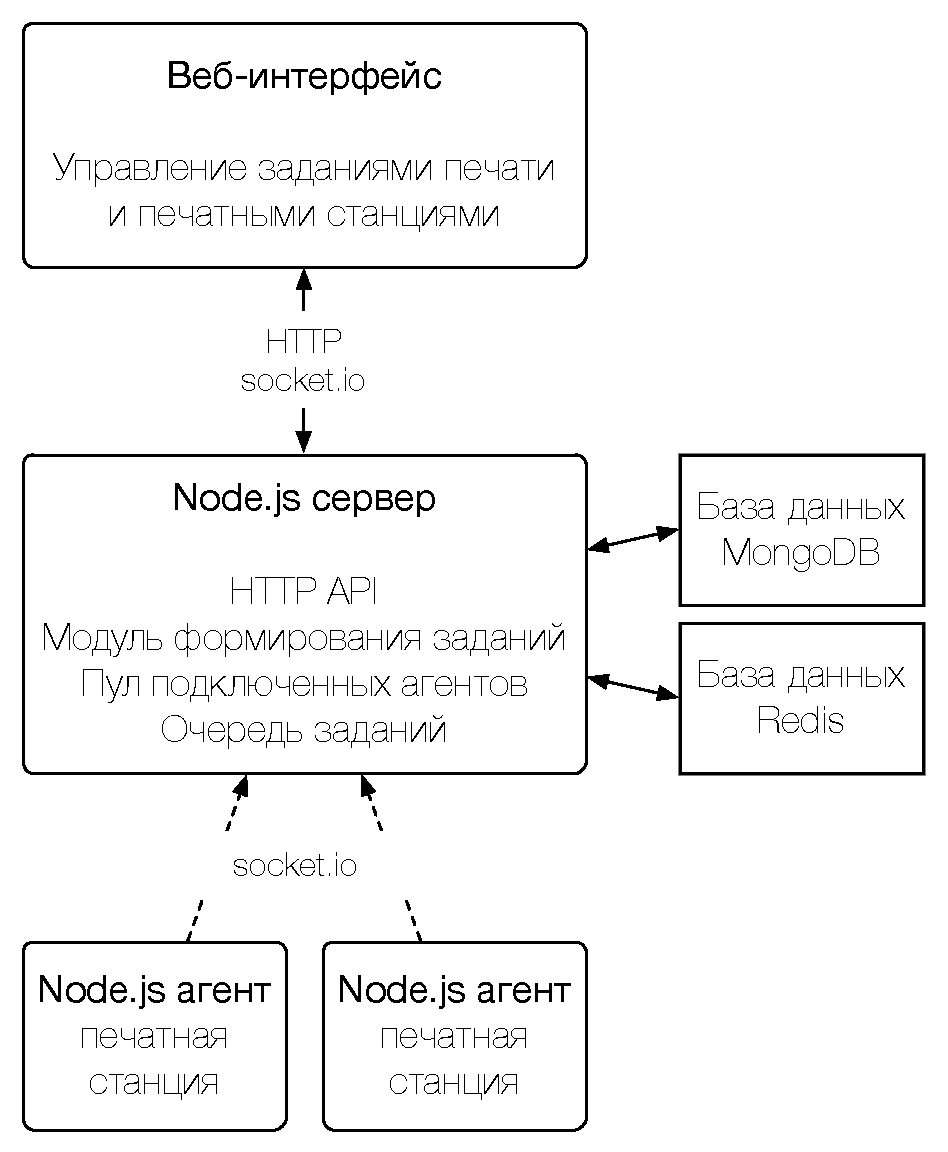
\includegraphics[scale=1.0]{architecture.pdf}
    \caption{Архитектура разработанного приложения}
    \label{fig:Architecture}
\end{center}
\end{figure}

Данный компонент написан с использованием со\-бы\-тий\-но--ориен\-тированного фреймворка \textit{node.js}\cite{nodejs}, в качестве языка программирования был выбран скриптовый язык JavaScript. Этот выбор был обусловлен наличием в языке средств функционального программирования (это позволяло при разработке делать максимальный упор на алгоритм) и его минималистичность. Кроме того, язык обладает рефлексивностью, что делает его незаменимым при написании программ с возможностью добавления сценариев (одна из отличительных черт программ для тестирования).

\begin{figure}[htbp]
\begin{center}
	\includegraphics[scale=0.95]{thread_map.png}
    \caption{Потоковая карта, построенная при помощи разработанного приложения}
    \label{fig:ThreadMap}
\end{center}
\end{figure}


\paragraph{Веб--интерфейс} Накопленная в результате тестов статистика отображается в веб--интерфейс программы посредством асинхронных \textit{http}--запросов, причем их обработка также происходит с помощью фреймворка \textit{node.js}. Это возможно благодаря встроенному в \textit{node.js} веб--серверу и дополнительным библиотекам\cite{expressjs}.

	Кроме того, была реализована возможность построения на стороне клиента потоковых карт пройденных тестов (рисунок \ref{fig:ThreadMap}). Потоковая карта --- это диаграмма работы потоков программы во времени, с проявившимися симптомами. При помощи таких карт возможнен чисто визуальных анализ результатов конкретного теста.

\subsection{Апробация методов}
  Для проверки работоспособности разработанного продукта был проведен ряд экспериментов, задачей которых был поиск ошибок некоторого программного обеспечения. Предприняты попытки поиска ошибок в следующих программах:\begin{enumerate}
\item \textit{WinDjView}\cite{WinDjView} (просмотрщик djvu--документов) --- применялся стохастический метод для генерации произвольного djvu--файла.
\item \textit{Tesseract}\cite{Tesseract} (программа для распознавания текста) --- применялся стохастический метод для генерации произвольного jpeg--файла, кроме части файла, отвечающей за начало заголовка.
\item \textit{Bmap}\cite{Bmap} (свободный просмотрщик изображений) --- применялся мутационный метод на основе выбранного jpeg--изображения. В качестве мутации рассматривалось произвольное изменение частей заголовка файла.
\item \textit{TinyImg}\cite{TinyImg}(свободный просмотрщик изображений, небольшой проект) --- применялась аналогичная мутация заголовка исходного bmp--изоб\-ра\-жения.
\end{enumerate}

	В ходе последнего эскперимента была выявлена ошибка, проявляющаяся в отсутствии проверки на размер изображения в заголовке bmp-изображения.

	Отсутствие найденных границ в первых трех случаях свидетельствует о соблюденных нормах контроля качества при разработке, что соответствует статусу проектов (разработка ведется на протяжении многих лет квалифицированными специалистами).
\newpage
\section*{Заключение}
\addcontentsline{toc}{section}{Заключение}
	В ходе проделанной работы были получены следующие результаты:
\begin{enumerate}
\item Разработано средство для автоматического стресс-тестирования программного обеспечения посредством входных файлов.

\item Реализованы стохастический и мутационный методы поиска граничных значений черного ящика.

\item При апробации средства были выявлены ошибки в одной из тестируемых программ, что подтверждает работоспособность реализованных методов.
\end{enumerate}

	Таким образом, тестирование является мощным средством для выявления ошибок в программном обеспечении, позволяя добиться стабильности, эффективности и надежного разрабатываемых продуктов.

Использование метода черного ящика делает возможным применение автоматизации при тестировании, что является альтернативой трудоемкого ручного поиска программных дефектов.

\newpage
\addcontentsline{toc}{section}{Список литературы}

\bibliographystyle{unsrt}
\bibliography{bibliography/sources}

\end{document}
